\documentclass[tikz,border=10pt]{standalone}
\usepackage{amsmath}
\usepackage{tikz}
\usetikzlibrary{decorations.pathmorphing}

\begin{document}

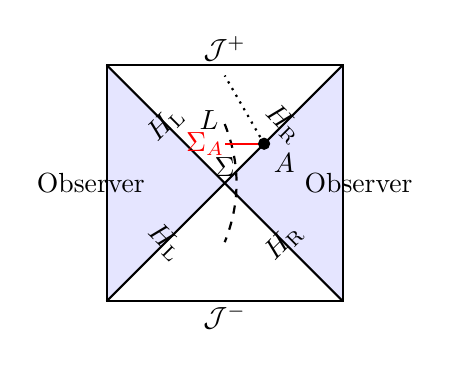
\begin{tikzpicture}

% Set up coordinates
\coordinate (A) at (1.5,1.5);
\coordinate (B) at (-1.5,1.5);
\coordinate (C) at (-1.5,-1.5);
\coordinate (D) at (1.5,-1.5);
\coordinate (E) at (0,0.75);
\coordinate (F) at (0,-0.75);

% Fill patches
\fill[blue!10] (B) -- (C) -- (0,0) -- cycle;
\fill[blue!10] (A) -- (D) -- (0,0) -- cycle;

% Draw horizon lines
\draw[thick] (B) -- (D);
\draw[thick] (C) -- (A);

% Draw spacelike slice
\draw[dashed, thick] (E) .. controls (0.2,0.25) and (0.2,-0.25) .. (F);

% Draw future lightsheet
\draw[dotted, thick] (0.5,0.5) -- ++(120:1);

% Draw segment Σ_A
\draw[red, thick] (0.5,0.5) -- ++(180:0.5);

% Draw dot for sphere A
\filldraw (0.5,0.5) circle (2pt) node[below right] {$A$};

% Labels
\node at (0,1.7) {$\mathcal{J}^+$};
\node at (0,-1.7) {$\mathcal{J}^-$};
\node[rotate=45] at (-0.75,0.75) {$H_{\rm L}$};
\node[rotate=-45] at (0.75,0.75) {$H_{\rm R}$};
\node[rotate=-45] at (-0.75,-0.75) {$H_{\rm L}$};
\node[rotate=45] at (0.75,-0.75) {$H_{\rm R}$};
\node at (-1.7,0) {Observer};
\node at (1.7,0) {Observer};
\node at (0,0.2) {$\Sigma$};
\node[red] at (-0.25,0.5) {$\Sigma_A$};
\node at (-0.2,0.8) {$L$};

% Draw box outline
\draw[thick] (B) -- (A) -- (D) -- (C) -- cycle;

\end{tikzpicture}

\end{document}